%%%%%%%%%%%%%%%%%%%%%%%%%%%%%%%%%%%%%%%%%
% baposter Landscape Poster
% LaTeX Template
% Version 1.0 (11/06/13)
%
% baposter Class Created by:
% Brian Amberg (baposter@brian-amberg.de)
%
% This template has been downloaded from:
% http://www.LaTeXTemplates.com
%
% License:
% CC BY-NC-SA 3.0 (http://creativecommons.org/licenses/by-nc-sa/3.0/)
%
%%%%%%%%%%%%%%%%%%%%%%%%%%%%%%%%%%%%%%%%%

% \title{CSAFE poster template}

%-------------------------------------------------------------------------
%	PACKAGES AND OTHER DOCUMENT CONFIGURATIONS
%-------------------------------------------------------------------------

\documentclass[landscape,a0paper,fontscale=0.275, margin = 25mm]{baposter} % Adjust the font scale/size here
\usepackage{setspace}
\usepackage{graphicx} % Required for including images
\graphicspath{{figures/}} % Directory in which figures are stored

\usepackage{amsmath} % For typesetting math
\usepackage{amssymb} % Adds new symbols to be used in math mode

\usepackage{booktabs} % Top and bottom rules for tables
\usepackage{enumitem} % Used to reduce itemize/enumerate spacing
\usepackage{palatino} % Use the Palatino font

\usepackage{natbib}

\usepackage[font=small,labelfont=bf]{caption} % Required for specifying captions to tables and figures

\usepackage{subcaption}
\usepackage{tabu}
\usepackage{enumitem} % Itemize separation
\setlist{nosep} % or \setlist{noitemsep} to leave space around whole list
\setitemize{nolistsep,leftmargin=*}

\usepackage{multicol} % Required for multiple columns
\setlength{\columnsep}{1.5em} % Slightly increase the space between columns
\setlength{\columnseprule}{0mm} % No horizontal rule between columns

\usepackage{tikz} % Required for flow chart
\usetikzlibrary{shapes,arrows} % Tikz libraries required for the flow chart in the template

\newcommand{\compresslist}{ % Define a command to reduce spacing within itemize/enumerate environments, this is used right after \begin{itemize} or \begin{enumerate}
\setlength{\itemsep}{1pt}
\setlength{\parskip}{0pt}
\setlength{\parsep}{0pt}
}

\definecolor{lightblue}{rgb}{0,0,0.4} % Defines the color used for content box headers
\definecolor{navyblue}{rgb}{0,0,0.4} % Defines the color used for content box headers
\definecolor{antiquefuchsia}{rgb}{0.57, 0.36, 0.51}
\definecolor{bananayellow}{rgb}{1.0, 0.88, 0.21}
\definecolor{bittersweet}{rgb}{1.0, 0.44, 0.37}
\definecolor{raspberry}{rgb}{0.89, 0.04, 0.36}

% This removes any blank page added in the beginning of a document
\usepackage{atbegshi}% http://ctan.org/pkg/atbegshi
\AtBeginDocument{\AtBeginShipoutNext{\AtBeginShipoutDiscard}}
\pretolerance=10000
\usepackage{hyperref}
\renewcommand{\figurename}{Fig.} % Shorten figure caption label
\begin{document}

\begin{poster}
{
%grid=true,
columns=3,
headerborder=closed, % Adds a border around the header of content boxes
colspacing=.8em, % Column spacing
bgColorOne=white, % Background color for the gradient on the left side of the poster
bgColorTwo=white, % Background color for the gradient on the right side of the poster
borderColor=lightblue, % Border color
headerColorOne=navyblue, % Background color for the header in the content boxes (left side)
headerColorTwo=lightblue, % Background color for the header in the content boxes (right side)
headerFontColor=white, % Text color for the header text in the content boxes
boxColorOne=white, % Background color of the content boxes
textborder=rectangle, % Format of the border around content boxes, can be: none, bars, coils, triangles, rectangle, rounded, roundedsmall, roundedright, roundedleft, or faded
eyecatcher=true, % Set to false for ignoring the left logo in the title and move the title left
headerheight=0.14\textheight, % Height of the header
headershape=rectangle, % Specify the rounded corner in the content box headers, can be: rectangle, small-rounded, roundedright, roundedleft or rounded
headerfont=\Large\bf, % Large, bold and sans serif font in the headers of content boxes
%textfont={\setlength{\parindent}{1.5em}}, % Uncomment for paragraph indentation
linewidth=2pt % Width of the border lines around content boxes
}
%-------------------------------------------------------------------------------
%	TITLE SECTION 
%-------------------------------------------------------------------------------
%
{
\includegraphics[height=7em]{logo.png}} % First university/lab logo on the left
{\huge\bf Validation studies for an automated bullet matching algorithm\vspace{0.3em}} % Poster title
{{\Large Heike Hofmann, Susan VanderPlas and Alicia Carriquiry, Iowa State University}\vspace*{-0.6em}} % Author names and institution
{
\includegraphics[height=5em]{logo-NIST.jpg}} % Second university/lab logo on the right

%---------------------------------------------------------------------------------
%	OBJECTIVES
%---------------------------------------------------------------------------------

\headerbox{Automated Bullet Matching}{name=objectives,column=0,row=0,boxpadding=2mm}{
\textbf{Background}
Automated bullet matching algorithms utilizing 3D scans have been described in many studies \citep{dekinderAutomatedComparisonsBullet1999,bachrachDevelopment3DbasedAutomated2002,xieAutomatedBulletidentificationSystem2009, chuPilotStudyAutomated2010}, using features such as cross-correlation \citep{maNISTBulletSignature2004, vorburgerApplicationsCrosscorrelationFunctions2011, chuPilotStudyAutomated2010} and consecutive matching striae \citep{chuAutomaticIdentificationBullet2013,biasotti}.\vspace{.25em}

The \textbf{Random Forest} \citep{breiman} \textbf{matching algorithm}  combines features derived from 3D topographic scans of land engraved areas \citep{aoas}, using the following steps:
\begin{enumerate}\compresslist\item Identify an area with expressed striae\item Discard degraded areas\item Remove bullet curvature\item Align signatures\item Calculate features: cross-correlation, striae depth, \# matching striae, CMS, Euclidian distance, and more\end{enumerate}
The RF model was fit to two Hamby sets (252, 173) from NBTRB scanned with a resolution of 1.5625 microns \citep{nist}\vspace{.25em}

\textbf{Goal} \begin{itemize}\item Validate \citep{aoas} on external test sets\item Assess sensitivity to distributional changes\item Examine limitations due to training data parameters\end{itemize}

Valid Scores should fulfill the following two criteria:
\begin{enumerate}
\item[(R1)] {\bf Monotonicity:} a higher score is indicative of higher similarity between a pair of bullets, in particular, similarity scores of same-source pairs of bullets are higher than different-source pairs.
\item[(R2)] {\bf Stability:} the same score leads to the same conclusion. 
\end{enumerate}
}

%----------------------------------------------------------------------------------------
%	CASE STUDIES
%----------------------------------------------------------------------------------------

\headerbox{Validation Sets}{name=sets,column=0,below=objectives,above=bottom,boxpadding=2mm}{ % This block's bottom aligns with the bottom of the references block
3 sets, increasingly different configurations and test materials:\vspace{.5em}
\begin{itemize}
\item {\bf Hamby 44}\citep{hamby} 2 $\times$ 10 known, 15 question, Closed\\{\footnotesize 10 Ruger P85 barrels, Winchester 9mm Luger 115 Grain FMJ}
\item {\bf Phoenix PD} 3 $\times$ 8 known, 10 question, Open\\{\footnotesize 8 Ruger P95 barrels, provided by Tylor Klep, Phoenix PD, scanned by Bill Henderson (Sensofar)}
\item {\bf Houston FSI} 3 sets: 3 $\times$ 5 known, 8 question, Open\\{\footnotesize 10 Ruger LCP barrels, Remington UMC 9mm Luger FMJ; provided by Melissa Nally and Kasi Kirksey, FSI Houston}
\end{itemize}\vspace{.5em}
Validation sets scanned with a Sensofar confocal light microscope (20x, 0.645 microns) - finer resolution than the training sets.
}

%----------------------------------------------------------------------------------------
%	Bullet-To-Bullet
%----------------------------------------------------------------------------------------

\headerbox{Bullet-To-Bullet Comparisons}{name=b2b,column=1,row=0,boxpadding=2mm}{ 
    \centering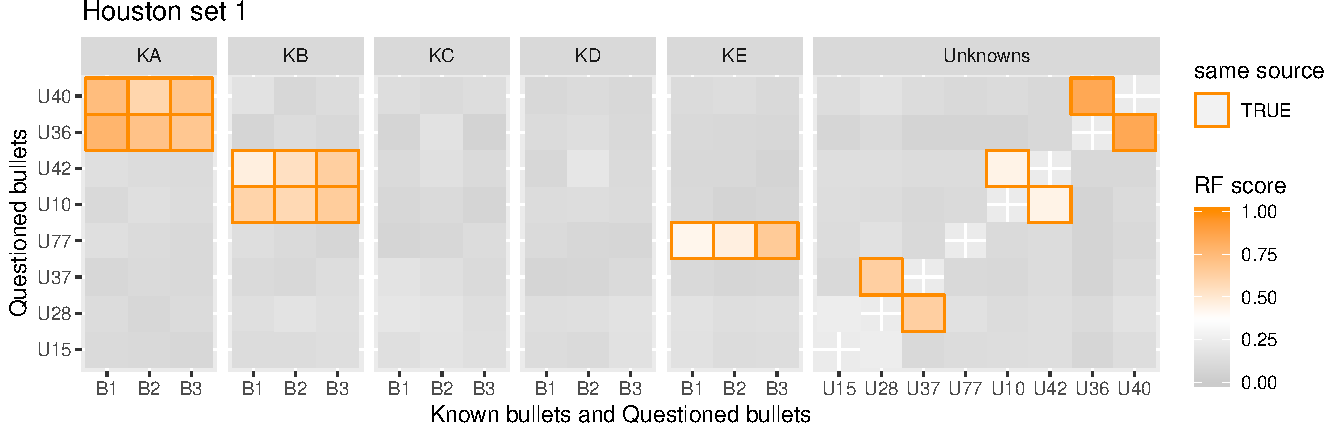
\includegraphics[width = .9\textwidth]{figures/hou-1.pdf}
    \captionof{figure}{Overview of matching scores for all pairs of questioned bullets to known bullets (left) and questioned bullets (right).}
%    \label{fig:hou1}
    \centering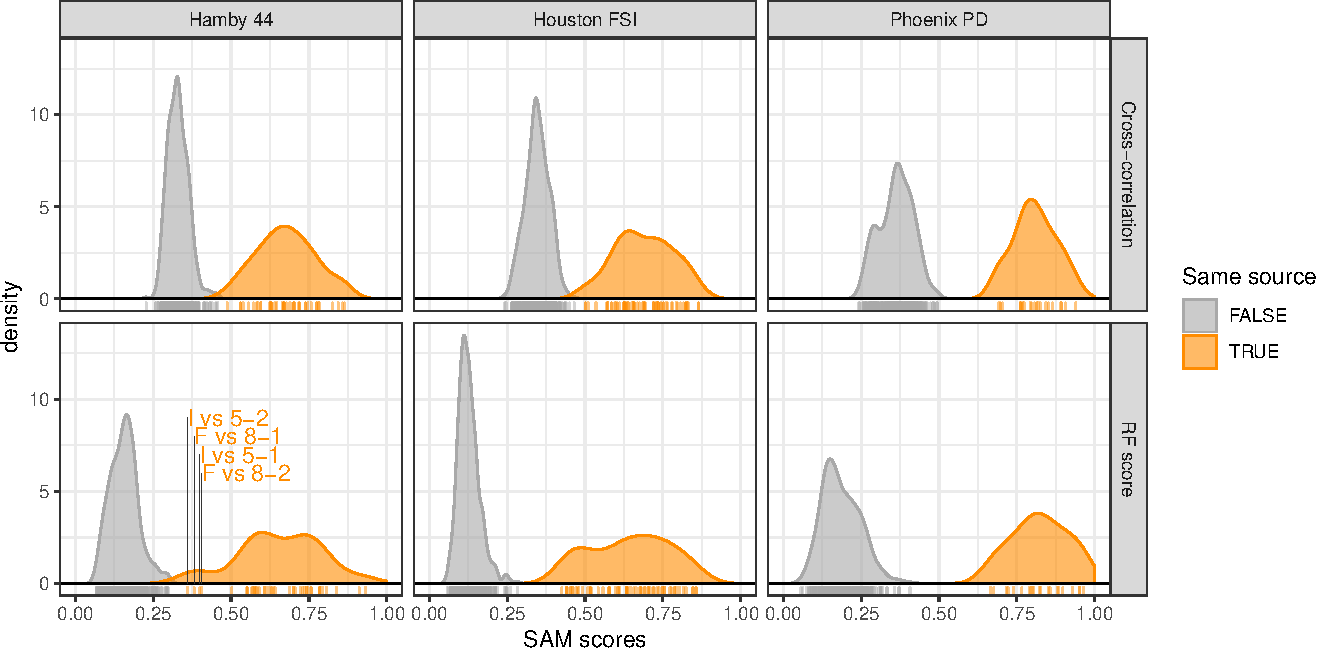
\includegraphics[width = \textwidth]{figures/compare-1.pdf}
    \captionof{figure}{Density curves of similarity scores from cross-correlation (top) and RF scores (bottom). Ideally all scores of different source pairs should be much lower than scores for same source pairs.}

}



%----------------------------------------------------------------------------------------
%	Applications
%----------------------------------------------------------------------------------------

\headerbox{Measurements}{name=other,column=1,span=1,below=b2b,above=bottom,boxpadding=2mm}{

Let $z(t)$ describe a signature. $z(t)$ forms a spatial process with location indexed by $t$ for  $t = 1, ..., T$, where $T$ is the number of pixels.\vspace{0.5em}
 
The Random Forest score, Cross-correlation and Consecutively Matching Striae are evaluated for each pair of signatures:

\begin{itemize}\compresslist
    \item[] \textbf{Cross-correlation}: for two signatures $x(t)$ and $y(s)$ the cross-correlation is defined as $\arg \max \rho_{XY}(\tau)$ with 
    \[
     \rho_{XY}(\tau) = \frac{1}{\sigma_X, \sigma_Y}
     E[(X_t - \mu_X)(Y_{t+\tau} - \mu_Y)]
    \]
    
    \item[] \textbf{Consecutively Matching Striae (CMS)} defined by \citep{biasotti}.\\ Generally, CMS of 6 or above is considered 'a match'.
\end{itemize}


}

%----------------------------------------------------------------------------------------
%	Land to Land
%----------------------------------------------------------------------------------------

\headerbox{Land-To-Land Comparisons}{name=l2l,column=2,row = 0,boxpadding=2mm}{
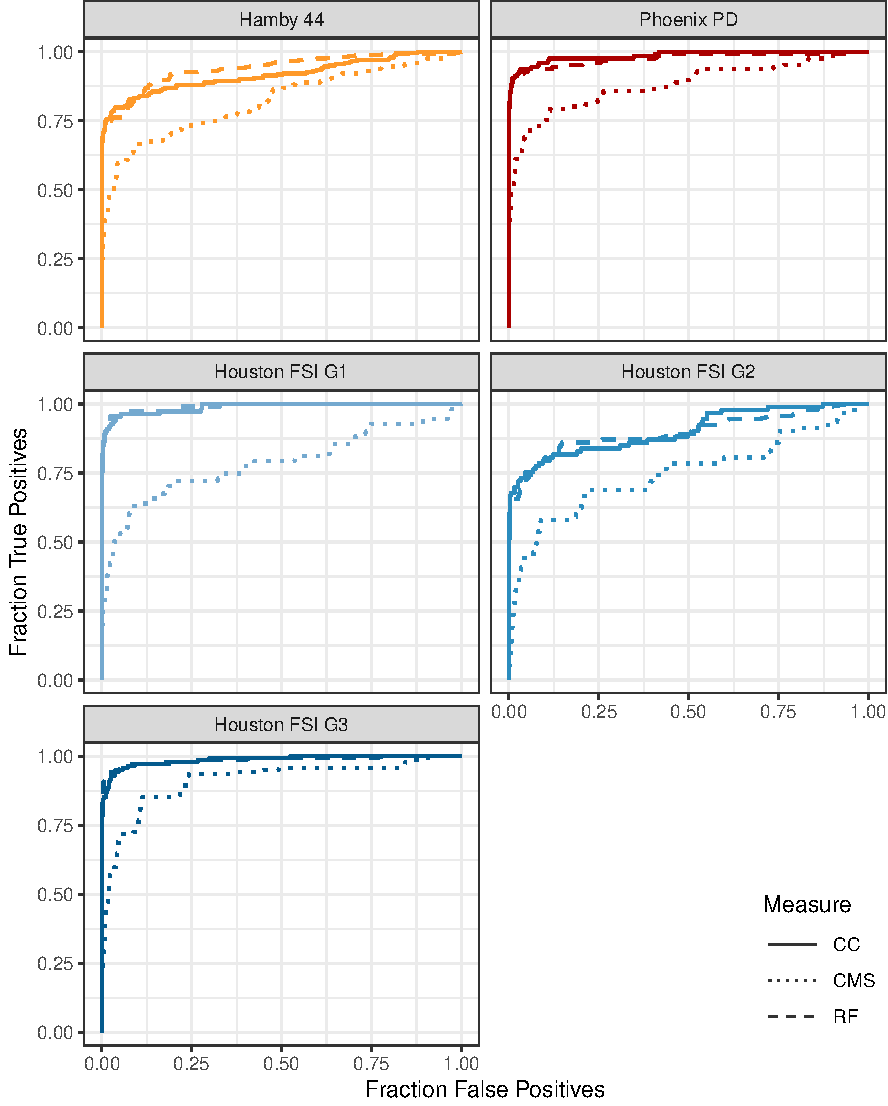
\includegraphics[width=.49\textwidth]{figures/roc-auc-1.pdf}\hfill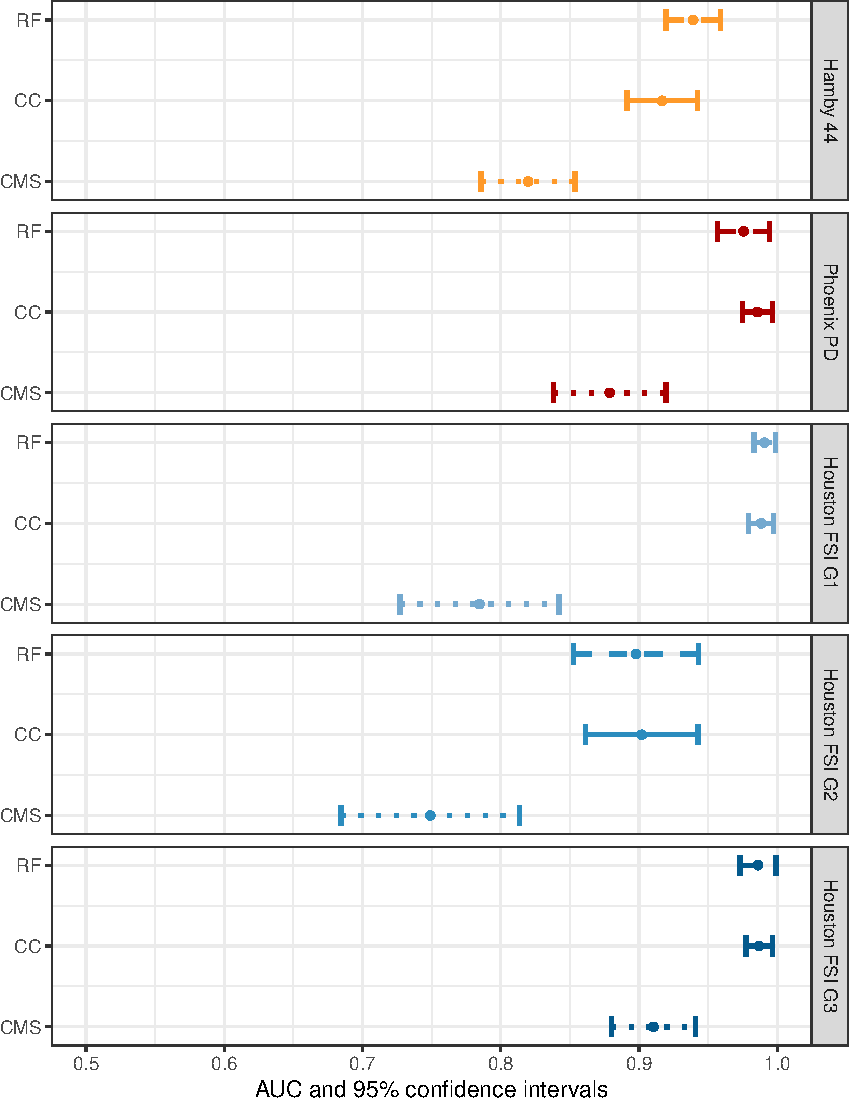
\includegraphics[width=.45\textwidth]{figures/roc-auc-2.pdf}\captionof{figure}{ROC curves and AUC values for each test set using cross correlation (CC), consecutive matching striae (CMS), and the random forest score (RF).}
}


%----------------------------------------------------------------------------------------
%	Applications
%----------------------------------------------------------------------------------------

\headerbox{Future Work}{name=fw,column=2,span=1,below=l2l,boxpadding=2mm}{
\vspace{.5em}
\begin{itemize}
\item Re-fit the random forest with sets of different resolutions, barrel make, manufacture, and ammunition types. 
\item Improve the ability to utilize partial signatures from bullets with tank rash and other damage
\item Investigate algorithm performance with more diverse barrels
\end{itemize}\vspace{.5em}
}


%----------------------------------------------------------------------------------------
%	REFERENCES
%----------------------------------------------------------------------------------------

\headerbox{References}{name=refs,column=2,row=1,span=1,below=fw,above=bottom,boxpadding=2mm}{
\renewcommand{\section}[2]{} % Get rid of the default "References" section title
\renewcommand{\bibfont}{\tiny}\setlength{\bibsep}{0pt plus 0.2ex}
\bibliographystyle{unsrt}
\bibliography{Refs} % Use sample.bib as the bibliography file
}




%----------------------------------------------------------------------------------------
% \headerbox{foot}{name=foot,column=0, span=4, above=bottom}{
% abcdefghijklmnop}
%\cfoot{abcdddddddddddd}


\end{poster}
{\vspace*{0.05em}\tiny{This work was partially funded by CSAFE through Cooperative Agreement \# 70NANB15H176 between NIST and Iowa State University, which includes activities carried out at Carnegie Mellon University, University of California Irvine, and University of Virginia}
\end{document}